This chapter tries to summarize the main applications of pixel detectors, while a description of the technological implementation is presented in chapter \ref{chap:pixel}; in the following sections I will also use terms such as hybrid pixels, monolitich active pixel systems (MAPS), Charge Coupled Devices (CCDs), Depleted Field Effect Transistor sensors (DEPFET) that will discussed later. 

The relation between the development of cameras and that of pixel detectors dates back to 1969, when the idea of CCDs, for which Boyle and Smith were awarded the Nobel Prize in Physics in 2009, revolutionized photography allowing light to be captured electronically instead of on film. 
Even though the CMOS technology already existed at the time the CCDs spread, the costs of productions were too high to allow the diffusion of these sensors for the following 20 years. From that moment on, the fast diffusion of CMOS was mainly due to the less cost than CCD, and the less power supply required. Nowadays CCDs are still prefered over MAPS in astronomy, where the astronomical sources' rate are low enough to cope with slow readout time (tens of \si{ms}).  

The principal use cases of pixel detectors in physics are particle tracking and imaging: in the former case individual charged particles have to be identified, in the latter instead an image is obtained by the usually un-triggered accumulation of the impinging radiation. 
%Also the demands on detectors performance depends on their usage, in particular tracking requires high spatial resolution, fast readout and radiation hardness. 

\section{Tracking in HEP}
    In the early days of high-energy physics gaseous detector where used for tracking and there was no need to replace them since they had a sufficient spatial resolution (\SI{100}{\um}). Since 1974, with the measurement of the invariant mass of the J/Psi and the affirmation of the quark model, all experiments start to look for better spatial resolutions in order to achieve the possibility of reconstructing short lived particles and measuring their decays length.  

    Historically\cite{cern_courier_2021}, the first pixel detector employed in particle physics was a CCD: it was installed in the spectrometer at the CERN’s Super Proton Synchrotron by the ACCMOR Collaboration (Amsterdam, CERN, Cracow, Munich, Oxford, RAL) in the mid 1980s, with the purpose of studying the (at the time) recently-discovered charmed particles.
    The second famous usage of CCDs took place in the SLAC Large Detector at SLAC linear collider in the years 1996-98, where the CCD technology was adopted instead of the microstrip detectors for their excellent spatial resolution (cell size 22$\times$22\si{\um\squared} giving a resolution of $\sim$\SI{5}{\um}) thanks to the sufficient time for readout between two successive collisions (\SI{160}{ms}).

    From that period on, particle tracking in HEP experiments has been transformed radically. It became mandatory to build a inner vertex detector, with the following tasks:
    \begin{itemize}
        \item pattern recognition with the identification of particle tracks even in the presence of large backgrounds and pile-up
        \item measurement of vertices (primary and secondary)
        \item multi-track and vertex separation in the core of jets
        \item measurement of specific ionization
        \item momentum measurement combining with the information from other detectors 
    \end{itemize}

    The more demanding requirements led to the development of hybrid pixel detectors starting from 1990s: a dedicated collaboration, RD19, was established at CERN with the specific goal of defining a semiconductor micropattern detector with an incorporated signal processing at a microscopic level. 
    In those years a wide set of prototypes of hybrid pixel has been manufactured; among the greatest productions a mention goes to the huge ATLAS and CMS vertex detectors. 
    From the middle of 2013 a second collaboration, RD53, has been established with the new goal of finding a pixel detector suitable for the phase II in future upgrades of those experiments. Requirements imposed by LHC are stingent and they will become even more with the increase of luminosity at HL-LHC: for example, a dose and radiation of \SI{500}{Mrad} and 10$^{16}$~MeV~n$_{eq}$/cm$^2$ are exepcted after 5 years of operation. Time resolution, material budget and power consumption are also issues for the upgrade: to distinguish different events from different bunches a time resolution better than \SI{25}{ns} for a bunch crossing frequency of \SI{40}{MHz} is required, a material budget lower than 2\% X$_0$ and a power consuption lower than \SI{500}{mW/cm\squared} are required. 

    Even if the collaboration is specifically focused oFn the design of hybrid pixel readout chips (aiming to \SI{65}{nm} tecnique), also other options have been taken in account per quanto riguarda the sensor. 
    Among the solutions proposed to improve radiation robustness of the sensor, 3D silicon detector, invented by Sherwood Parker in 1995, are very promising.
    In 3D sensors the electrode is a narrow column of n-type implanted vertically across the bulk instead of being implanted on the wafer's surface. 
    The charge produced by the impinging particle is then drifted transversally within the pixel, and, as the mean path between two electrode can be soufficent low, the trap probability is not an issue. 
    Even if 3D detector are adequately radiation hard and are a possible solution for hybrid pixel modules, especially in the innermost pixel detector layer, their fabrication process is currently low volume, making them unlikely to cover large areas.
    Another promising possibility is to use fast Monolitich Active Pixels systems which could allow the reduction of material budget and improve spatial resolution.


    \subsection{Hybrid Pixels at LHC}
    \subsubsection{ATLAS}    
        \begin{figure}
                \centering
                \begin{subfigure}[b]{0.49\textwidth}
                    \centering
                    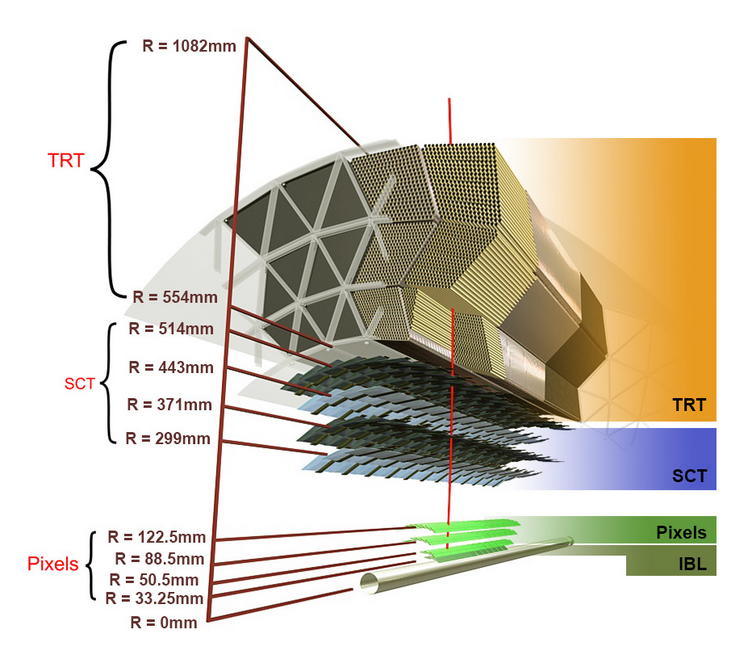
\includegraphics[width=\linewidth]{figures/pixel_detectors_usage/ATLAS.png}                
                    \caption{ATLAS tracker detector}
                    \label{fig:ATLAS}
                \end{subfigure}
                \hfill
                \begin{subfigure}[b]{0.49\textwidth}
                    \centering
                    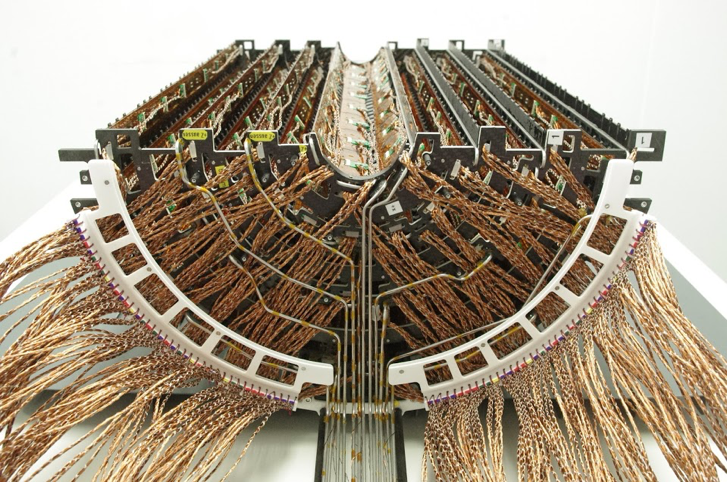
\includegraphics[width=\linewidth]{figures/pixel_detectors_usage/cms.png} 
                    \caption{CMS barrel pixel detector}
                    \label{fig:CMS}
                \end{subfigure}
                \caption{}
                \label{fig:ATLAS_CMS}
        \end{figure}
        ATLAS is one of two general-purpose detectors at the LHC and has the largest volume detector ever constructed for a particle collider (\SI{46}{m} long and \SI{25}{m} in diameter).  
        The Inner Detector (ID) consists of three different systems all immersed in a magnetic field parallel to the beam axis whose main components are: the pixel, the micro-strips and transition radiation trackers (fig.\ref{fig:ATLAS}). 
        Concerning the pixel detector, they installed a 3-layer hybrid pixel detector in 2007 and an additional one inserted within the original detector envelope and therefore called insertable B-layer (IBL) in 2014.
        92 million pixels are divided in 4 barrel layers and 3 disks in each end-cap region, covering a total area of \SI{1.9}{m\squared} and having a \SI{15}{kW} of power consumption. 

        As stated by the ATLAS collaboration the pixel detector is exposed by an extreme particle flux: "By the end of Run 3\footnote{Run 3 start in June 2022}, the number of particles that will have hit the innermost pixel layers will be comparable to the number it would receive if it were placed only a few kilometres from the Sun during a solar flare". Considering that the particle density will increase even more with HL-LHC, radiation hardness is definitively a target to achieve. 
        Also the complexity of the readout will be raised, as the number of pixels will be increased of a factor about 7, passing from 92 milions to 6 billion, then a readout logic will have to meet the high amount of data. 

        Hybrid pixels will be used at the start of high-luminosity application, although an active development of monolitich devices is ongoing for possible future use in the outer pixel layers. The TJ-Monopix1 which I will describe in chapter \ref{chap:Monopix_Arcadia} is part of this development. 
       
        Regarding the sensor, a valueable option is using 3D pixels, which have already proved themselves in ATLAS, for the IBL, where they were introduced in a limited acceptance range; the sensor chosen for the upgrade will be bonded with ITkPix, the first full-scale \SI{65}{nm} hybrid pixel-readout chip developed by the RD53 collaboration.


        %3D silicon sensor technology has been chosen to instrument the innermost pixel layer of ITk, which is the most exposed to radiation damage. 50  50 and 25  100 .D
        %sensors are an established technology that has been already
        %employed in experiments at the LHC such as in the ATLAS
        %Insertable B-Layer (IBL)  and for the tracker of the AFP
        %experiment . With respect to these designs the new ITk 3D
        %sensors feature a reduced pixel cell size of 25  100 and 50 
        %50 um 2 with one collecting electrode .  active substrate of these new
        %sensors is reduced to 150 um in comparison to the previous
        %generation of 230 um thick 3D sensor
        \subsubsection{CMS}
        The CMS hybrid pixel detector (fig.\ref{fig:CMS}) has been upgraded in 2017, when, with the replacement of a piece of the beam pipe, a layer has been added to the detector at \SI{3}{cm} from it.
        124 million pixels are divided between the barrel pixel detector (BPIX) and the forward disks (FPIX), with sensors which are different from each other and produced by different foundryes. 
        The sensors have an area equal to \SI{100}{\um} by \SI{150}{\um} and have been produced on \SIrange{285}{300}{\um} thick wafers.
    
        The time resolution is \SI{25}{ns}, the rate capability  \SI{600}{MHz/cm\squared}, and the information coming from the detector are stored on chip for the Level-1 trigger latency ($\sim$\SI{4}{\us}). The upgrade ROIC was redesigned for the outer 3 layers, replacing analog signal readout with on-chip ADCs which record the pulse height information or with digital readout at higher rate. 

        \subsubsection{LHCb}
        LHCb is a dedicated heavy-flavour physics experiment that exploits pp interactions at \SI{14}{TeV} at LHC. 
        It was the last experiment to upgrade the vertex detector, the Vertex Locator (VELO), replacing the silicon-strip with 26 plane pixel detector (beacause of the fixed target geometry) in May 2022. 
        As the instantaneous luminosity in Run3 is increased by a factor $\lesssim$10, much of the readout electronics and of the trigger system have been developed in order to cope with the large interaction rate.
        To place the detector as close as possible to the beampipe and reach a better track reconstruction efficiency and resolution, the VELO has a surprising feature: during the injection of LHC protons it is parket at \SI{3}{cm} from the beams and only when the stability is reach it is moved at $\sim$\SI{5}{mm}. Readout speed is a priority for the detector that use a triggerless readout at \SI{40}{MHz} collision rate, producing \SI{20}{Gbps} per ROIC. 
        The Velopix, which is the hybrid system designed for LHCb, is made by bonding sensors, each measuring 55$\times$55 micrometers and \SI{200}{\um}-thick, to a \SI{200}{\um}-thick ASIC specially developed for LHCb and coming from the Medipix family, which can handles hit rates up to \SI{900}{MHz} per chip. 
        Since the detector is operated under vacuum near the beam pipe, the heat removal is particularly difficult and evaporative CO2 microchannel cooling are used. 

    \subsection{Monolitich Active Pixels}
    \subsubsection{MIMOSA}
    \begin{figure}
            \centering
            \begin{subfigure}[b]{0.49\textwidth}
                \centering
                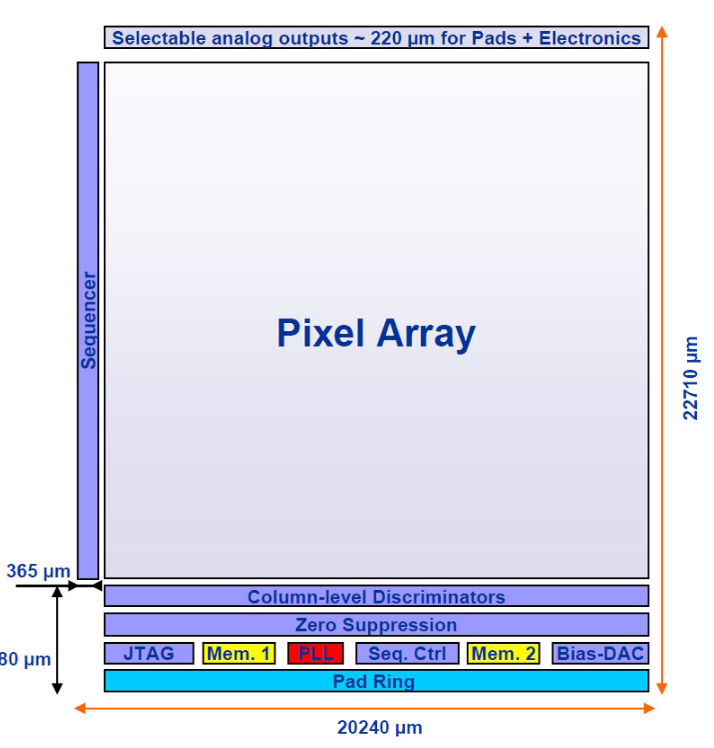
\includegraphics[width=\linewidth]{figures/pixel_detectors_usage/MIMOSA.png}          
                \caption{Block-diagram of the ULTIMATE-2 sensor of the MIMOSA family}
                \label{fig:MIMOSA}
            \end{subfigure}
            \hfill
            \begin{subfigure}[b]{0.49\textwidth}
                \centering
                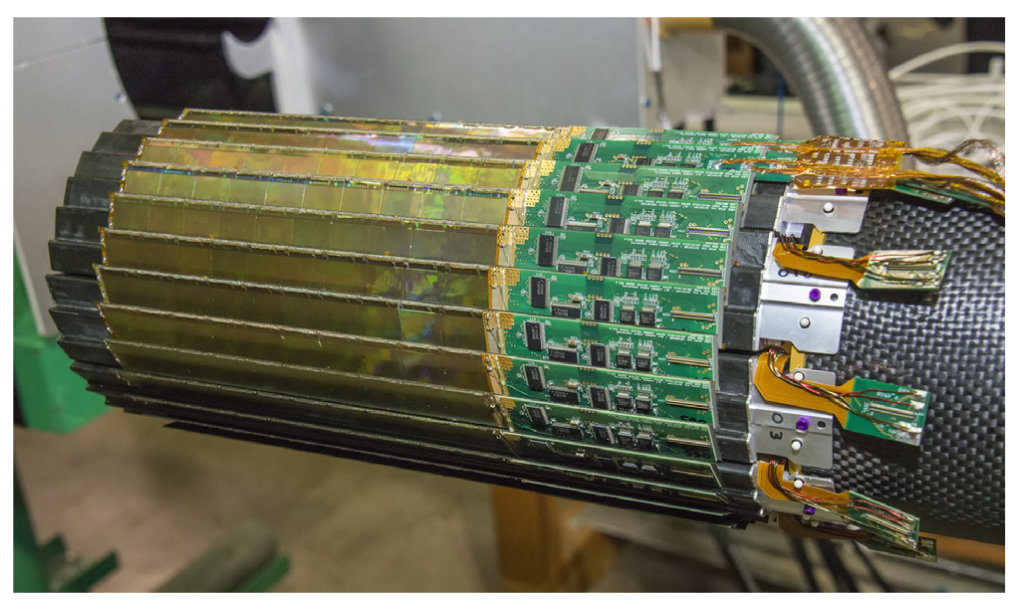
\includegraphics[width=\linewidth]{figures/pixel_detectors_usage/STAR.png}
                \caption{The HFT pixel detector of STAR}
                \label{fig:HFT}
            \end{subfigure}
            \caption{}
            \label{fig:EUDET_STAR}
       \end{figure}
        MIMOSA \cite{MIMOSA}\cite{MIMOSA26} (standing for Minimum Ionizing MOS Active pixel sensor), designed in 2008, prefigured the architecture of MAPS for coming vertex detector being the first large scale sensor to be employed as detector. MIMOSA-26 equiped the final version of EUDET high resolution  beam telescope both at CERN-SPS and at DESY while the MIMOSA-28 devices are used for the first MAPS-based vertex detector at the STAR experiment at RHIC.
        MIMOSA-26 is fabricated in a \SI{350}{nm} CMOS technology, and a module features 1152 columns, split into 18 indipendent groups, and 576 rows, with square pixels having a side of \SI{18.4}{\um} lenght; the epitaxyal layer is not fully depleted and the charge collection is mostly by diffusion, resulting in charge sharing between pixels and collection time bigger than \SI{100}{ns}.
        The chip is an Active Pixel Sensor (APS) and therefore it incorporates on pixel the amplification, while the signal discrimination and zero-suppression logic are placed at the End of Column: the readout is done in a rolling shutter mode with a frame integration time that can be lowered down to \SI{85}{ms}, moreover a memory allows to store up to six hits. 

        The EUDET telescope, equipped with six sensor planes, requires high granularity and thin pixel detectors in order to achieve an excellent track resolution (around \SI{2}{\um}) even at the rather low particle energies of \SI{6}{GeV}.
        The STAR experiment at the Relativistic Heavy Ion Collide (RHIC) accelerator at the Brookhaven National Laboratory (BNL) is the first to include MAPS in the vertex detector\cite{STAR}.
        The main tracking detector in STAR is a TPC with radii 60-190 cm  embedded in a \SI{0.5}{T} solenoidal magnetic field, that provides a pointing resolution of approximately \SI{1}{mm}. 
        The pixel detector, PXL, is a part of a 3-detector system, the Heavy Flavor Tracker (HFT), and has been added to the pre-existing STAR apparatus just before the 2014 Run in order to improve the impact parameter resolution and to enable the direct reconstruction of hadronic decays of heavy flavor mesons and baryons.     
        The Heavy Flavor Tracker (fig.\ref{fig:HFT}) is composed by the Silicon Strip Detector, the Intermediate Silicon Tracker and the Pixel Detector (PXL); the first one is placed at \SI{22}{cm} from the beam pipe and consists of double sided strips with \SI{95}{\um} inter-strip pitch, the second one, placed at \SI{14}{cm}, is made of single sided silicon pads with \SI{600}{\um}$\times$\SI{6}{mm} pitch and the last one made by two layes is placed at \SI{2.8}{cm} and \SI{8}{cm} fabricated with ULTIMATE-2\ref{fig:MIMOSA} (also known as MIMOSA-28), a successor of MIMOSA-26 sensor, with pitch \SI{20.7}{\um} and thinned down to \SI{50}{\um} (fig.\ref{fig:MIMOSA}).
        An area of \SI{0.16}{m\squared} is covered by 400 MAPS sensor, corresponding to 356 milions of pixels divided into array size of 928 $\times$ 960.
        Each pixel includes circuitry for readout, amplification, and Correlated Double Sampling for signal extraction and noise subtraction and the frame integration time is \SI{185.6}{\us}; after the subtraction the signal to noise ratio is $\sim$ 30, with a noise between 10-12 electrons and a signal of \SI{1000}{\elementarycharge ^-}.
        Thanks to the Heavy Flavor Tracker system and the Pixel Detector, STAR achieved a track pointing resolution of \SI{46}{\um} for \SI{750}{MeV/c} kaons, and better than \SI{30}{\um} for particle momenta bigger than \SI{1}{GeV/c}: this performance enabled the study of D-meson production with a high significance signal.

        Another possible application of MIMOSA has been proposed by ALICE, which has been studing the possibility of exploiting the extreme granularities of MAPS for calorimeter application\cite{review_calo}. In a such calorimeter, the energy measurement would come out from the counts of particles traversing the active layers, resulting then in a digital calorimeter. A prototype forward calorimeter (FoCAL), fabricated with the MIMOSA23 chips and containing 39 million pixels devided in 24 layers, alternated with 24 layers of tungsten (\ref{fig:ALICE_FoCAL}), have been tested with electron beams and exhibited an energy resolution better than standard hadronic calorimeters, with a stochastic terms of 30\%/$\sqrt{E(GeV)}$, a constant term of 2.8\% and noise term of \SI{0.063}{GeV}.

        \subsubsection{ALPIDE at ALICE}
        \begin{figure}
            \centering
            \begin{subfigure}[b]{0.6\textwidth}
                \centering
                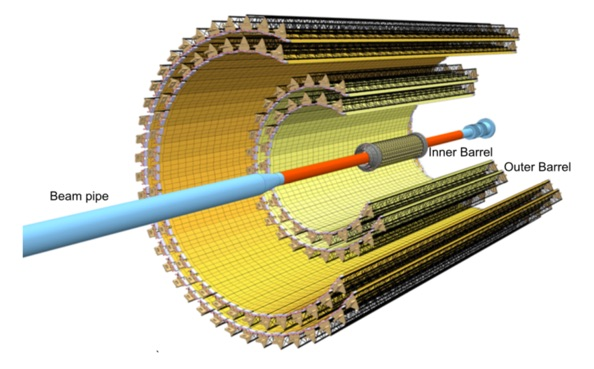
\includegraphics[width=\linewidth]{figures/pixel_detectors_usage/alice.png}        
                \caption{ALICE ITS scheme}
                \label{fig:ALICE_ITS}
            \end{subfigure}
            \hfill
            \begin{subfigure}[b]{0.39\textwidth}
                \centering
                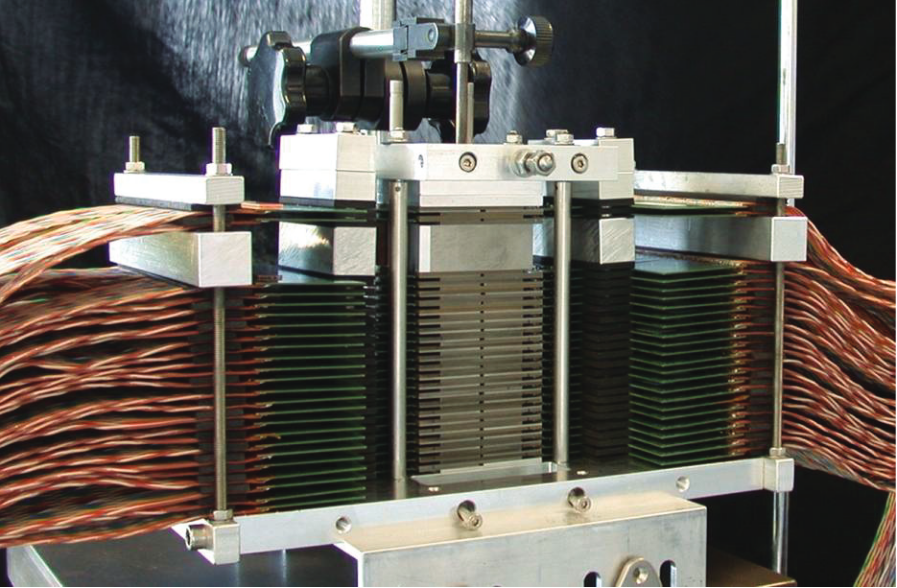
\includegraphics[width=\linewidth]{figures/pixel_detectors_usage/ALICE_FoCAL.png}
                \caption{FoCAL prototype fabricated with MAPS}
                \label{fig:ALICE_FoCAL}
            \end{subfigure}
            \caption{}
            \label{fig:ALICE_RD}
       \end{figure}
        
        The ALICE (A Large Ion Collider Experiment) tracking detector consists of the Inner Tracking System (ITS), the gaseous Time Projection Chamber (TPC) and the Transition Radiation Detector, all embedded in a magnetic field of \SI{0.5}{T}. The ITS (fig.\ref{fig:ALICE_ITS}) is made by six layers of detectors, two for each type, from the interaction point outwards: Silicon Pixel Detector, Silicon Drift Detector and Silicon Strip Detector.         
        Contrary to the others LHC experiments, ALICE tracker in placed in a quite different environments, which enables the usage of a MAPS-based detector: the dose assorbed by the tracker is expected to be smaller by two order of magnitude and the rate of interactions is few \si{MHz} instead of \SI{40}{MHz}, even though the number of particles coming out from each interaction is very high (the Silicon Pixel Detector is invested by a density of particles of $\sim$\SI{100}{\per cm\tothe{-2}}).  
        The reconstruction of very complicated events with a large number of particle is then a challenge, hence to segment and to minimize the amount of material, which may cause secondary interaction futher complicating the event topology, is considered a viable strategy. 
        
        ITS2, upgraded during the LHC long shut down in 2019-20, was the first large-area ($\sim$10 \si{m\squared} covered by 2.5 Gpixels) silicon vertex detector based on CMOS MAPS.
        The detector employes the ALPIDE chip, developed by ALICE collaboration, fabricated in the \SI{180}{nm} CMOS Imaging Sensor process of TowerJazz, whose design takes full advantage of process feature which allows full circuitry within the pixel matrix.
        Thanks to the reduction in the material budget, ITS2 obtained an amazing improvement both in the position measurement and in the momentum resolution, especially improving the efficiency of track reconstruction for particle with very low transverse momentum (by a factor 6 at p$_{T}$$\sim$\SI{0.1}{GeV/c}). Further advancements in CMOS MAPS technology are being aggressively pursued for the ALICE ITS3 vertex detector upgrade (foreseen around 2026-27), with the goals of reducing the sensor thickness and improving the readout speed (which now is completely asynchronous) of the devices, while keeping power consumption at a minimum.

        \subsubsection{BelleII}
        \begin{figure} 
            \centering
            \includegraphics[width=0.77\linewidth]{figures/pixel_detectors_usage/Belle2.pdf}      
            \caption{BelleII vertex detector}
            \label{fig:Belle2_Vertex}
       \end{figure}

        Due to the high background level coming from the nanobeam used at SuperKEKB in order to achieve a such high luminosity (6$\times$10$^{35}$\si{/cm\squared/s}), silicon strip cannot be used in the inner layer of the tracker. The occupancy is too high to allow the usage of strips up to \SI{40}{mm} from the beam pipe. 
        Moreover for a precise reconstruction of B-decay vertices, the usage of thin detector is mandatory at the low energy (4-\SI{7}{GeV}) of the beam, in order to minimize the multiple scattering of particles. 
        The current Vertex Detector of BelleII, VXD, is made of a Pixel Detector (PXD), fabricated with 2 layers of DEPFET-based pixels, and 4 layers of a double-sided silicon strip detectors (SVD)\cite{BelleII-DEPFET}.
        Due to the small capacitance of the collection node, DEPFET presents a high signal-to-noise ratio (in 30-50) thanks to the low instrinsic noise and to the large signal achieved with he fully depleted bulk: pixels are thinned to \SI{75}{\um} in the active region, then a Minimum Ionizing Particle (MIP) is expected to create a signal of $\sim$\SI{6000}{\elementarycharge ^-} (eq.\ref{eq:charge_MIP}), while the typical noise of DEPFET is around \SI{200}{\elementarycharge ^-}.
        The ASIC read out is still based on a rolling shutter logic, with an integration time of \SI{20}{\us}.
        In order to reduce the data-storage memory PXD hits are only used to improve spatial resolution of tracks: the SVD informations are used by the High Level Trigger to look for regions of interest in the pixel ladders just by extrapolating back the tracks found in the tracker detector, and this method allows to store only data belonging to these areas; the PXD hits are then used in offline track fit to improve the vertex resolution.
        
        CMOS MAPS have been proposed for the replacement of VXD during the  Long Shut Down 2 foreseen around 2026-27; the new vertex detector, VTX, should be made of 5 layers fabricated with the optimized Belle II pixel sensor (OBELIX), a detector based on TJ-Monopix (see at chapter \ref{chap:Monopix_Arcadia}).    
        The main advantages VTX should bring are a significant improvment in the track and vertex resolution (\SI{14}{\um} before upgrade, $\lessapprox$\SI{10}{\um} expected after upgrade), a reduction in the material budget, a higher background tolerance because of the smaller sensor than strips dimension.

\section{Other applications}
    Pixel detectors are widely used also for photon detection: they can be used as single photon counter or integrating and collecting the charge released by more impinging particles. The utilisation in the first case is similar to the tracking one, except that the requirements are less tight, so much that two noteworthy of microchips originally meant for detectors in particle physics at the LHC, and later employed in other fields are Medipix and Timepix. They are read-out chips developed by the Medipix Collaborations since early 1990s. For two decades, different Medipix generations have been produced, having a rough correlation with the feature size used: for example, Medipix2 (1999) used \SI{250}{nm} feature size CMOS while Medipix3 (2005) \SI{130}{nm}.
    For photons imaging other materials with higher atomic charge than silicon could be prefered, as a high photon absorption efficiency is needed: it was for this reason that Medipix2 was bump bonded to identically segmented sensors of both Si and GaAs.\cite{KOSTAMO2008174}
    
    The applications in scientific imaging vary from astrophysics and medical imaging to more exotic domains as studies of protein dynamics, material science, art authentication and archaeology.
    One of the most important employment of Medipix is as X-ray single photon counting in industrial and medical radiography and in 3D computed tomography\footnote{The analysis of the direction dependence of X-ray absorption is perform, for example, in order to obtain an image in Computed Tomography (CT)}. Regarding the latter, for example, thanks to a New-Zealand company, the MARS Bioimaging detector has been fabricated, which is capable of resolving the photons energy and produce 3D coloured images.
    Besides tracking in HEP (I have already cited the use of Timepix3 is in the beam telescope of the LHCb VELO), an important use of Timepix is in dosimetry.
    \red{Timepix Detector for Imaging in Ion Beam Radiotherapy- articolo e qualche info.}
    A small-Timepix detector with the dimension of a USB can also be found at the International Space Station, where it is exploited for radiation, principally made of haevy-ion, monitoring. 
 
    \subsection{Applicability to FLASH radiotherapy}
        A possible new application of pixels detector is dosimetry or beam monitoring of charge particles in high intensity radiotherapy (RT).
        Recently\footnote{The first evidences has been observed on a mice experiments in 1966 and in 2014 by the group of Favaudon and Vozenin. After this, many test on cats and pigs have been performed, and also there has been a clinical trial on a cutaneous tumor-patient} a promising method for radiotherapy at ultra high dose rate (at least \SI{40}{Gy/s}) and for this reason called FLASH-RT\cite{FLASH_review}, instead of CONV-RT (\SI{0.03}{Gy/s}), came out. However, finding dosimeters, as well as beam monitor, suitable at ultra high dose rate is still an open issue since almost all standard online dosimeters have shown saturation problems. In table \ref{tab:dose_parameters} are listed the typical value of operation which distinguish  between CONV-RT and FLASH-RT.

        \subsubsection{Radiotherapy}
            \begin{figure}
                \centering
                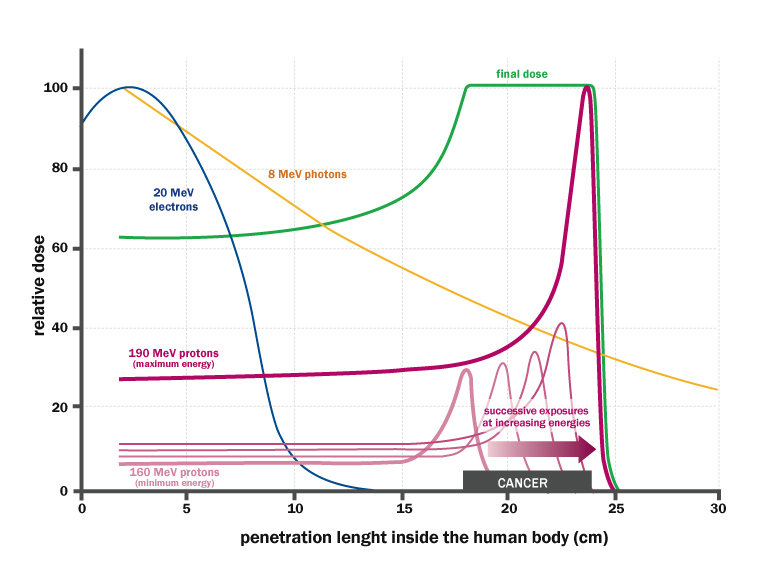
\includegraphics[width=.7\linewidth]{figures/pixel_detectors_usage/Bragg-Peak.png}
                \caption{The Spread Out Bragg Peak (SOBP) curve (green), which is a constant dose distribution, is obtained from the superposition of many Bragg peak of hadrons with different energy.}
                \label{fig:Bragg-peak}
            \end{figure}
            The radiological treatment is a common method used in 60\% of tumors both as palliative care and as treatment. It can be given before, after or during a surgery, (Intra operative radiation therapy-IORT) and many different types of radiations (photons, electrons, protons and ions, which mainly are carbon ions) can be used to irradiate the affected tissues.
            Exploiting the ionizating energy loss, that can be parametrized by the Linear Energy Transfer (LET), a biological damage can be delivered to the tissue: while protons, $\alpha$ particles and light ions are high LET radiations with values in range \SIrange{100}{200}{keV/\um}, x-rays and gamma-rays are low LET radiations with values in range \SIrange{0.2}{2}{keV/\um}.
            If x-ray photons, with energy in 4-\SI{25}{MeV} are used, the ionization is caused by the Compton electrons and pair production, and is more in the superficial layers of the tissue due to the exponential attenuation of the beam. 
            The heavy charged particles energy loss, instead, is strongly localized in the final region of the track, that is the Bragg peak, such as the the treatement typically requires the scanning of the target.
            
            Electrons, instead, of energy in range of a dozen of \si{MeV} tend to spread out on a bigger region of a few centimeters in both the diameter and thickness and for this reason using Very High Energy Electrons (VHEE) has been taken into account for irradiation of deeper tissues.

        \begin{table}
            \begin{center}
            \begin{tabular}{|c | c |c |}
            \hline
            & CONV-RT & FLASH-RT \\
            \hline
            \hline
            Dose rate & \SI{0.03}{Gy/s} & \SI{40}{Gy/s}\\
            Intra pulse dose rate & \SI{100}{Gy/s}&\SI{10 6}{Gy/s}\\
            Treatment duration & $\sim$minutes & $\lessapprox$\SI{500}{ms} \\
            Dose Per Pulse & \SI{0.3}{Gy} & \qtyrange{1}{10}{Gy}\\
            Pulse width & \SI{3}{\us} & $\sim$\SI{2}{\us} \\
            \hline
            \end{tabular}
            \caption{Typical range of values used in a CONV radiotherapeutic treatement made with pulsed beam, compared to the range in which the FLASH effect has been observed.}
            \label{tab:dose_parameters}
            \end{center}
        \end{table}

        \subsubsection{FLASH effect}
            \begin{figure}
                \centering
                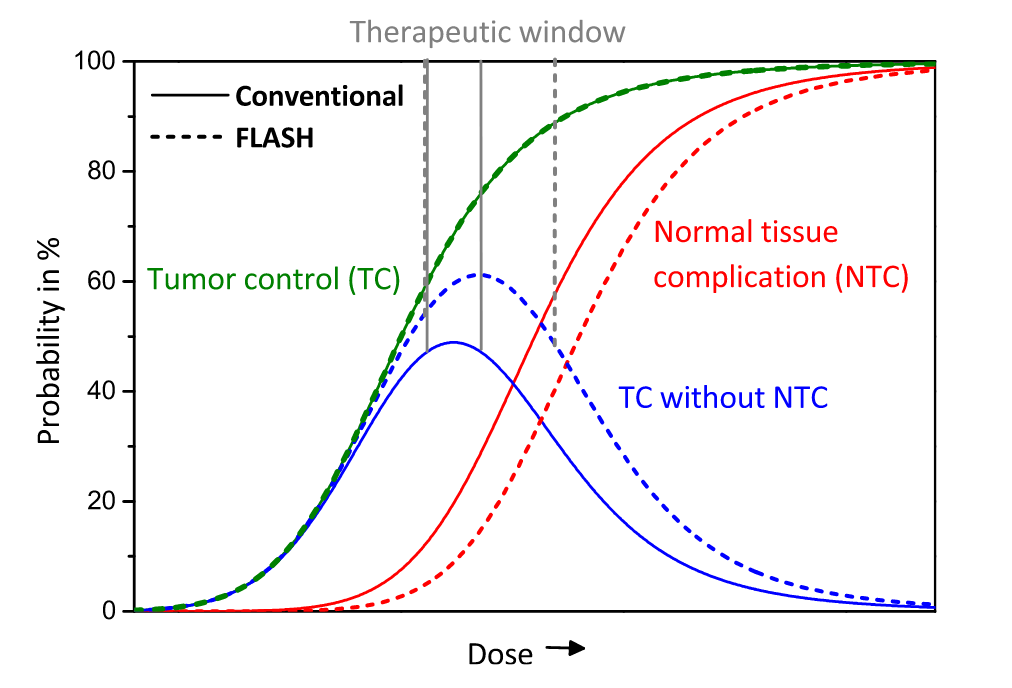
\includegraphics[width=.7\linewidth]{figures/pixel_detectors_usage/curve_flash.png}
                \caption{Illustration of dependence of Tumor Control Probability (TCP), Normal Tissue Contral Probability (NTCP) and therapeutic window on dose, for CONV-RT ad FLASH-RT.}
                \label{fig:therapeutic_window}
            \end{figure}
            This treatment takes advantages of biological differences between tumors and healthy tissues: it is characterized by reducing normal tissue toxicity and maintaining equivalent tumor damage. 
            The response to dose can be described by the survival fraction probability, describing the fraction of surviving cell as a function of the dose: 
            \begin{equation}
                S(D) = S(0)\;e^{-( \alpha D \, + \, \beta D^2)}
                \label{eq:survival_curve}
            \end{equation}
            where $\alpha$ and $\beta$ respectively represents the rate of cell killing by single ionizing events and by double hits. 
            Hence, at high doses the density of damages increases and the cells repair becomes more difficult. 
            The FLASH effect is not yet completelly understood and the underlying mechanisms are not yet clear, but many ideas have been proposed; among the most debated there are the fact that the high dose rate would prevent cells from reparing, or that the cell oxygen content and the immune response play a role.
            However what has been noticed is that the FLASH-RT allows to widen the therapeutic window, defined as below. 
            The Tumor Control Probability (TCP) and the Normal Tissue Complication (NTC) functions parametrize respectively the efficiency of damaging on the tumor after having released a certain dose and the probability of affecting the healthy tissues. The intermediate zone between the increase of the TC and of the NTC is called therapeutic window, and the wider it is and the more effective the treatment. 


        \subsubsection{Dosimetric problems}
            Since the dosimeters problems are strictly related with the time structure of the beam used for the treatement, let's consider the case of a pulsed electron beam (fig.\ref{fig:beam_structure}), where a high quantity of dose ($\gtrsim$\SI{1}{Gy/pulse}) is released in a very short time (macropulses).            
            At small macro-pulse frequency the signal collection time is shorter than the time between pulses, and, consequently, the saturation is influenced only by the Dose Per Pulse (DPP).
            \begin{figure}
                \centering
                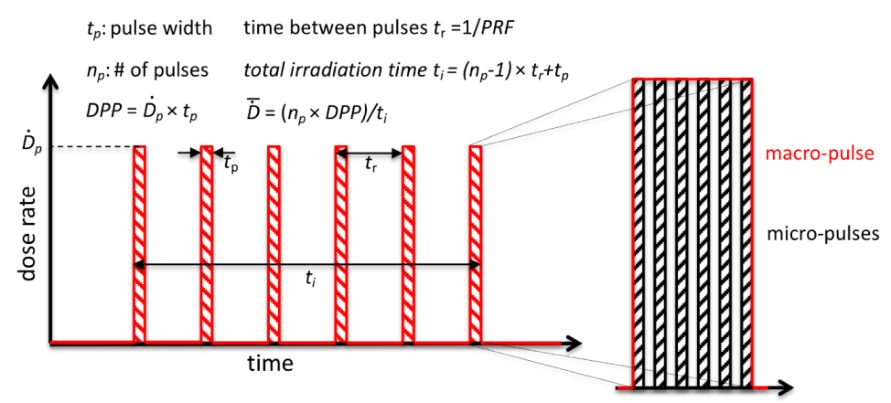
\includegraphics[width=.9\linewidth]{figures/test_beam/beam_structure.pdf}
                \caption{Typical beam structure of a beam used in electron radiotherapy}
                \label{fig:beam_structure}
            \end{figure} 
                    
            Up to now, all online dosimeters have shown saturation problems at high DPP, differently from radiochromic films, which are the standard passive dosimeters and have shown a dose-rate indipendece up to \SI{100}{Gy/s}.
            In spite of the response is linear in a wide dynamic range, they do not provide any online dosimetric informations, since the time required to extract the physical value from the reading is not long, requiring a measurement of the film density\footnote{The radiation produces a polymerization of an active layer, resulting in a different density of coloration.}.

            Ionization Chambers (ICs), which are the online reference dosimeter also according to law protocols, at high level of radiation (already at dose per pulse two orders of magnitude lower than the ones used for FLASH-RT) show both problems of saturation and recombination. When a high density of ions and electrons is produced in the gas, a high counter electric field opposed to the drift one might be generated; if a neutral region build up, both the recombination of i/e pairs, with a subsequent photoemission and abrupt discharge can happen. A correction factors, $k_{sat}$, can be introduced for sufficient low level of radiation and in this case a precise dose measurement can still be done: under conventional operation, with Dose Per Pulse lower than \SI{1}{mGy} the correction factor is $<$5\%. 

            Concerning the conventional semiconductor, if exposed to high dose rate, they suffer of saturation problems just as the ICs, but the development of fast MAPS devices, with rate capability of \SI{100}{MHz/cm\squared} or more, might open the possibility of using these detectors as dosimeters at high dose rates. 
            The idea is to use the high readout speed to split the dose per pulse in many buckets to reduce the saturation effect.
            Indeed a thin planar sensor could allow for the preservation of an enough strong electric field even at high dose rate which, together with the short mean path the e/h must cover to get the electrode (the epitaxial layer typically is $\sim$\SI{30}{\um}), could result in a fast collection of electrons by drift and in a non-saturated response.
            Besides, also the small capacity typical of MAPS is beneficial for reducing the readout time: a reduced C$_d$ enables for a fast discharge and then for a fast readout. 
            Finally, MAPS devices would provide good time and space resolutions compared to other dosimeter technologies, and since they can be thinned down to about \SI{50}{\um}, could also be employed in monitoring the beam position with minimal disturbance.
            
            Among  other detectors, optical fiber and alanine dosimeters have been proposed for high dose environments and many groups are going on studies on their applicability on FLASH-RT.  
            In reference \cite{FLASH_dosimeters} are presented some results related with saturation problems at high DDP of different types of detectors. The dosimeters tested and their value at which saturation becomes are reported in table \ref{tab:dosimeters_saturation}, while in figure \ref{fig:saturation_dosimeters} are reported the measurements. 
            The DrR is then defined as the ratio between the signal response of each dosimeters at a fixed DPP of \SI{1}{cGy/p} and is called dosimeter reading ratio (DrR): 
            \begin{equation}
                DrR = \frac{R}{R|_{Dp = 1cGy/p}} = \frac{R}{R_{ref}}
            \end{equation} 
            Then, for a saturation not affected by saturation problems DrR should be a straight line with a slope equal to 1; since the  reference measurements of dose has been performed with radiochromic films (GAFCHROMIC EBT-XD), whose dose indipendece has been tested\footnote{The radiochromic films calibration has been obtained by irradiating the films with dose values in range from \SIrange{0.01}{15}{Gy}, by positioning the films in a polymethylmethacrylate (PMMA) phantom at R$_{100}$ depth, corresponding to \SI{10}{cm}} in range from \SIrange{0}{15}{Gy}, the dotted black line in figure \ref{fig:saturation_dosimeters} represents the reference measurment done with it. 
            \begin{table}
                \begin{center}
                \begin{tabular}{|c | c |c |}
                \hline
                Commercial detector & Detector type & saturation [Gy/p]\\
                \hline
                \hline
                PTW TW34045 Advanced Markus EC & ionization chamber & 0.3 \\
                PTW TM60017 Dosimetry Diode E & silicon diode & 0.15\\
                PTW TW60019 microDiamond & diamond  &  0.15 \\
                DoseVue DoseWireTM Series 100 & scintillator fiber & 11-26\\
                \hline
                \end{tabular}
                \caption{Results obtain in \cite{FLASH_dosimeters}}
                \label{tab:dosimeters_saturation}
                \end{center}
            \end{table}
            \begin{figure}
                \centering
                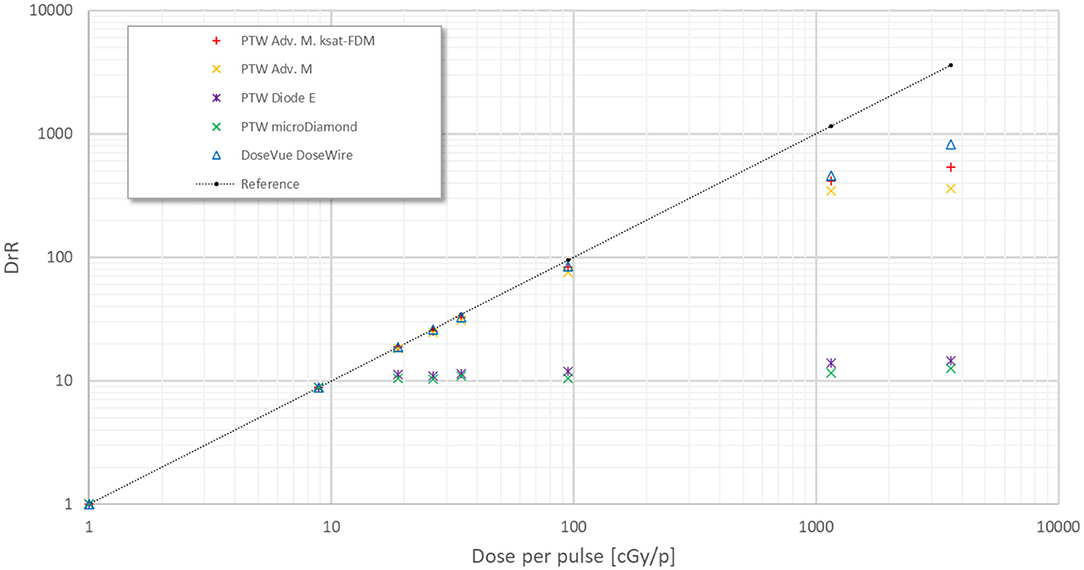
\includegraphics[width=.95\linewidth]{figures/pixel_detectors_usage/saturation1.png}
                %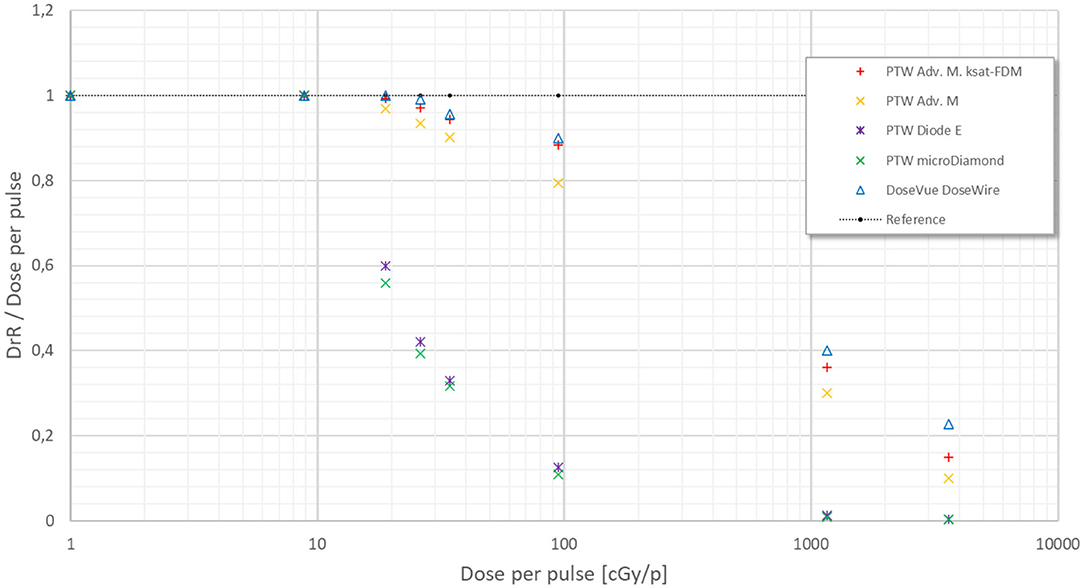
\includegraphics[width=.9\linewidth]{figures/pixel_detectors_usage/saturation2.png}
                \caption{Saturation problems underlyed in \cite{FLASH_dosimeters}. }
                \label{fig:saturation_dosimeters}
            \end{figure}            
            
